\chapter{Composition}

\section{Architecture}

\begin{figure}[here]
\centering
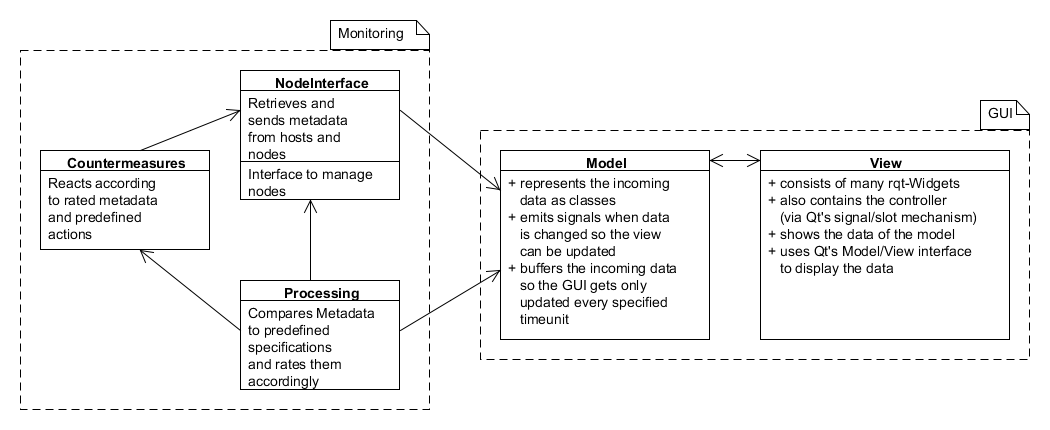
\includegraphics[scale=0.5]{./bilder/architektur.png}
\caption{architecture}
\label{fig:architecture}
\end{figure}

Figure ~\ref{fig:architecture} shows the general architecture of our software. It is divided into two parts, one for the graphical user interface and one for the monitoring aspect.
The right part depicts the GUI. It is designed using the MVC architecture, consisting of the usual three elements: model, view and controller. It will handle user-interaction.
The left part depicts the monitoring aspect. It consists of three elements : NodeInterface, Countermeasure and Processing. It will take care of collecting metadata, processing it and taking appropriate action in case of an error.

\subsection{Monitoring}

\begin{description}
	\item[NodeInterface]
		\begin{itemize}
			\item Retrieves and sends metadata from hosts and nodes
			\item Interface to manage nodes
		\end{itemize}
	\item[Processing] Compares Metadata to predefined specifications and rates the accordingly
	\item[Countermeasures] Reacts according to rated metadata and predefined actions	
\end{description}

\subsection{GUI}

\begin{description}
	\item[Model]
	\item[Controller]
	\item[View]
\end{description}